\documentclass{article}
\usepackage{amsmath, amssymb, mdwlist, graphicx, hyperref}
\usepackage{listings,color}
\usepackage{wrapfig}
\usepackage[usenames,dvipsnames]{xcolor}
\definecolor{gray}{rgb}{0.97,0.97,0.97}
\lstset{%
language=Python,%
%backgroundcolor=\color{gray},
emph={putpixel},
emphstyle=\bf,
tabsize=4,
framesep=5pt,
mathescape=true,
xleftmargin=2cm,
xrightmargin=2cm,
frame=lines,
%basicstyle=\ttfamily,
%keywordstyle=\color{Blue},
%commentstyle=\color{OliveGreen},
%stringstyle=\color{MidnightBlue},
columns=flexible,
%showstringspaces=false
}

\newcommand{\mpar}[1]{\marginpar{\textit{#1}}}
\newcommand{\norm}[1]{\Vert #1 \Vert}
\DeclareMathOperator{\argmax}{argmax}
\DeclareMathOperator{\argmin}{argmin}
\newenvironment{solution}{\paragraph{Solution.}$\,$ }{\vskip 3mm\hrule}
\newenvironment{exercise}[2]{\begin{verse}\textbf{Exercise #1 (#2pt).} }{
\end{verse}\medskip}
\newcommand{\bbR}{\mathbb{R}}
\newcommand{\bw}{\mathbf{w}}
\newcommand{\bx}{\mathbf{x}}
\newcommand{\bd}{\mathbf{d}}
\newcommand{\bb}{\mathbf{b}}
\newcommand{\by}{\mathbf{y}}
\newcommand{\bzero}{\mathbf{0}}
\newcommand{\bz}{\mathbf{z}}
\newcommand{\bSigma}{\mathbf{\Sigma}}
\newcommand{\bp}{\mathbf{p}}
\newcommand{\bP}{\mathbf{P}}
\newcommand{\bm}{\mathbf{m}}
\newcommand{\bc}{\mathbf{c}}
\newcommand{\bM}{\mathbf{M}}
\newcommand{\bV}{\mathbf{V}}
\newcommand{\bK}{\mathbf{K}}
\newcommand{\bD}{\mathbf{D}}
\newcommand{\bA}{\mathbf{A}}
\newcommand{\bX}{\mathbf{X}}
\newcommand{\bY}{\mathbf{Y}}
\newcommand{\bR}{\mathbf{R}}
\newcommand{\bI}{\mathbf{I}}
\newcommand{\bS}{\mathbf{S}}
\newcommand{\bT}{\mathbf{T}}
\newcommand{\balpha}{\boldsymbol{\alpha}}
\newcommand{\pt}[2]{\left(\begin{array}{c}#1\\#2\end{array}\right)}

\begin{document}
\title{MTAT.03.015 Computer Graphics (Fall 2013)\\
Exercise session V: Projection \& Vertex Shaders}
\author{Konstantin Tretyakov, Ilya Kuzovkin}
\date{October 7, 2013}
\maketitle

Today we shall study the vertex transformation from world space to clip space in detail. First we focus on its final step -- the projection transform, and then look at how the complete transformation can be specified using vertex shaders. As usual, the base code is provided in the \texttt{practice05.zip} archive on the course website or via the course github page. Download, unpack and open it. You will need to submit your solution as a zipped archive file.

\section{Clip Volume Normalization}
Projection is the last step of the vertex transformation (\emph{vertex shading}) pipeline. In classical OpenGL it can be specified using a $4\times 4$ \emph{projection matrix} $\bP$, that is applied to vertices right after the model-view matrix $\bV\bM$. That is, given the vertex with original homogeneous coordinate vector $\bx$, it is transformed to \emph{normalized device coordinates} $\bx_{\text{nd}}$ as follows:
$$
\bx_{\text{nd}} =\bP\bV\bM\bx\,.
$$

After this transformation, everything that falls into the cube $[-1, 1]\times [-1, 1]\times [-1, 1]$ is rendered onto the screen using standard 2D rasterization methods.

It is convenient to visualize the projection transformation in terms of the \emph{clip volume} that it imposes on the scene. That is, the original volume that will be mapped to the $[-1,1]\times [-1,1]\times [-1,1]$ cube after projection.

To understand this concept, open and run the project \verb#1_ClipVolume#. The application shows a simple scene rendered on the top left, the three dimensional view of the clip volume from a distance (bottom left) and the view of the normalized clip space after projection (bottom right). Use the spacebar to change between different projections. Examine the shape of the clip volume before projection, after projection, and see what happens to the vertices within the clip volume during projection.

\begin{exercise}{1}{0.5}
The three different projections are described in the functions \verb#scene_<xxx>_projection#, using OpenGL matrix multiplication routines. Currently, the function \\
\noindent
\verb#scene_perspective_projection# uses a call to \verb#gluPerspective# to specify the view frustum. Replace this with a call to \verb#glFrustum#, that would result in exactly the same clip volume.
\end{exercise}

\begin{exercise}{2*}{0.5}
Implement the function \\
\noindent \verb#scene_inverse_perspective_projection#. It should specify an \emph{inverted} perspective. That is, the view frustum should be exactly like the one of the original perspective, but with the front wider than the back. As a result, the dimensions of objects on the rendered scene will be \emph{greater} for objects further away from the camera. The picture you should aim for is shown below.
\begin{center}
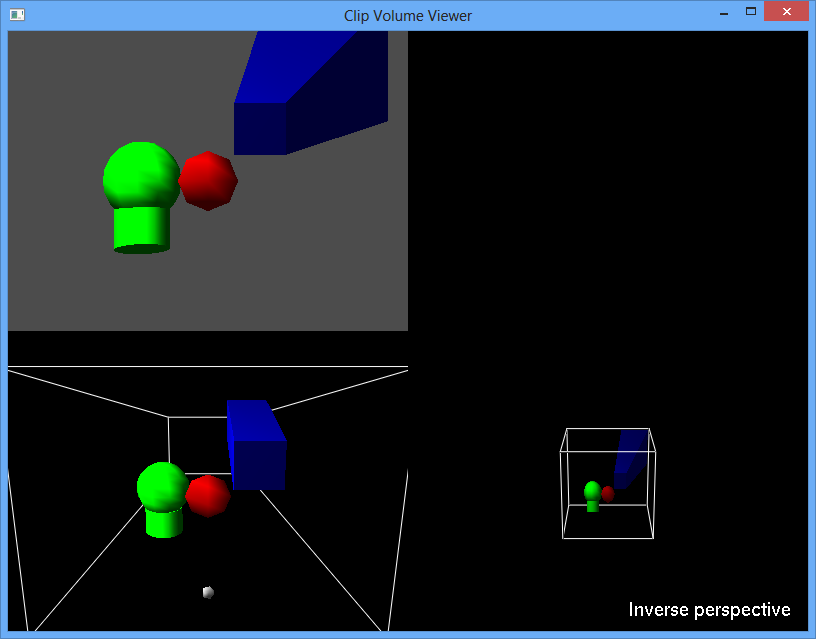
\includegraphics[width=0.8\textwidth]{inverseperspective.png}
\end{center}
\end{exercise}

\newpage
\begin{exercise}{3}{0.5}
The top-right viewport of the screen is currently free. We shall use it to implement a \emph{cross-eyed}\footnote{\url{http://www.starosta.com/3dshowcase/ihelp.html}} 3D view of the scene. Render into that viewport the same scene as is rendered in the top-right viewport, but with the camera rotated slightly to the left around the center of the scene (which is $(0, 0, -5)$ in camera coordinates). The result should look as shown below.
\begin{center}
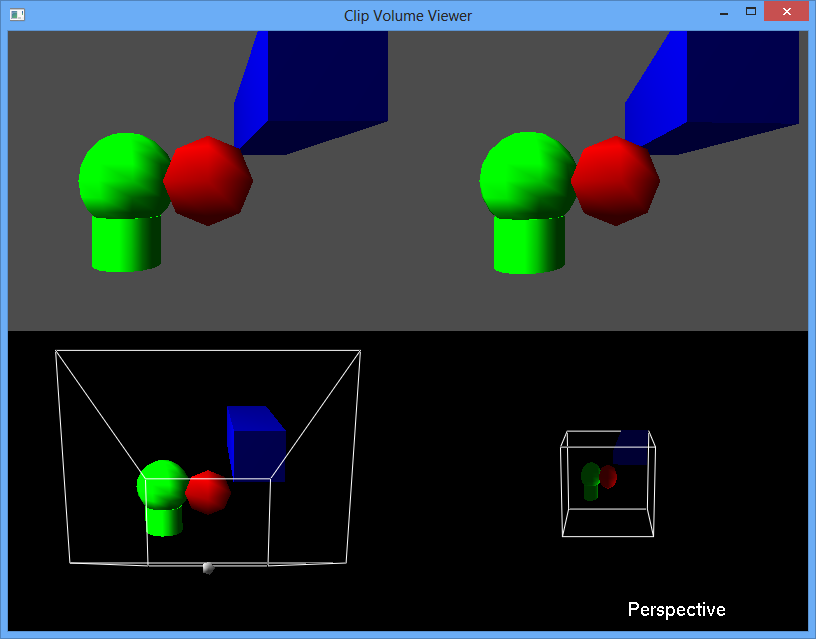
\includegraphics[width=0.8\textwidth]{crosseye.png}
\end{center}

Hint: If the use of \texttt{glViewport} and \texttt{glScissor} is not clear from the already existing code, do not hesitate to read the docs.
\end{exercise}

\begin{exercise}{4*}{1}
You should notice that the objects are colored differently in the lower right window: for perspective and inverse perspective projections the objects seem to be darker than in all other renderings. Explain why it is the case.

Hint: To solve this task you need to know that the colors of the vertices are determined by their position relative to the light source. The light source position is specified by the \texttt{glLightfv} line in the code (you'll have to find it and understand what is happening). Try changing the light position to be behind the camera and see what happens.
\end{exercise}

\section{Vertex Shading and GLSL}
The procedure of vertex transformation into clip space is known as \emph{vertex shading}, and can be customized in all modern graphics cards. The customization is done by providing a \emph{shader program}, that has to be written in a special C-like language -- \emph{GLSL}, the \emph{GL Shading Language}.

Open the project \verb#2_HelloGLSL# and study its structure. Although it should remind you the simplest GLUT ``Triangle'' program from the last week, there are three important changes.

\begin{enumerate}
\item Firstly, the project uses the GLEW library in addition to GLUT. \emph{GLEW (GL Extension Wrangler)} is necessary to enable the cross-platform use of most OpenGL features beyond the most basic ones. GLEW is enabled in a program by doing three simple things:
\begin{itemize}
\item Writing \verb@#include <GL/glew.h>@ in your program.
\item Invoking \verb#glewInit()# during initialization.
\item Adding \verb#glew32# (Windows) or \verb#GLEW# (Linux, Mac) to the list of libraries to link with (in the \emph{Build Options} dialog).
\end{itemize}
Once it is done, you can automatically use all of the newer OpenGL functions, supported by your graphics card.

\begin{verse} \textbf{Note:} The Windows version of the GLEW library is bundled with the base code. Linux users, please install the library by doing something like 
\begin{verbatim}
     sudo apt-get install libglew-dev
\end{verbatim}
(or equivalent). Mac users should do  
\begin{verbatim}
     sudo port install glew
\end{verbatim}
\end{verse}
\item Secondly, the project consists of more than one source file. Besides\\ \verb#hello_glsl.cpp#, which contains the main code of the program, there is \verb#shader_util.cpp#. This file has some useful functions and classes, which you do not need to worry about. Note, however, that the \emph{declarations} of those functions and classes are given in a separate \emph{header file}, \verb#shader_util.h#. This file is \verb@#include@-d in the main program, which lets you use the functions, just like you do with system libraries.

\item Finally, and most importantly, there is a separate file, \verb#simple_vertex_shader.glsl#, which contains the code for the custom vertex shader program in GLSL. This shader is loaded and enabled in the \verb#display# function using the code:
\begin{verbatim}
shader_prog shader("../src/simple_vertex_shader.glsl", NULL);
shader.use();
\end{verbatim}
\end{enumerate}

\subsection*{GLSL Basics}
Study the code in \verb#simple_vertex_shader.glsl#. You will see something, that resembles a tiny C program. This is GLSL, a limited version of C. The shader operation must be specified in the function \verb#main#. Within this function you may use basic arithmetics, declare variables, use \texttt{if}, \texttt{for} and \texttt{while} constructs, etc, just like in C. Besides the basic types (\texttt{int}, \texttt{float}, etc) there is a number of built-in data structures and functions for working with vectors and matrices. A nice description of them is given here: \url{http://en.wikibooks.org/wiki/GLSL_Programming/Vector_and_Matrix_Operations}.

The aim of a vertex shader is to compute the transformed position of a single vertex. The input vertex is provided in the built-in \emph{input} variable\footnote{\url{http://www.opengl.org/wiki/GLSL_Predefined_Variables_By_Version\#Vertex_shader_attributes}} \verb#gl_Vertex#. The transformed value must be saved into the built-in \emph{output} variable \verb#gl_Position#. The built-in function \verb#ftransform()# implements the default fixed-function model-view-projection transformation.

A number of other useful variables are available\footnote{Later versions deprecated most of them, though, in favor of manual variable binding.}. The variable\\ \verb#gl_ModelViewProjectionMatrix#, for example, is the model-view-projection matrix that you constructed in your OpenGL code.

Besides built-in variables, you can provide your own data to the shader from the program. In general, there are differences in how it is done depending on the kind of data\footnote{\url{http://www.opengl.org/wiki/Type_Qualifier_(GLSL)}}, but in this practice we shall only study a simple example of a \emph{uniform} variable (you are suggested to read the manual about \emph{in} variables too, though).

A \emph{uniform} variable is a variable that is common to all the vertices. You first need to declare it in the shader using the \texttt{uniform} keyword (check out the third line in the GLSL file). Then you have to bind the data from your program to this variable using functions \texttt{getUniformLocation} and \texttt{setUniform<xxx>} (check out the commented out code in the \texttt{display} function).

\begin{exercise}{5}{1}
Play with the code provided in \\ \noindent\verb#simple_vertex_shader.glsl#. Try uncommenting the different possibilities and see how they affect the result. To get the points for the task, change the shader so that the vertices would follow some funny trajectory, in the spirit of the last example shown there. For example, make them crawl along the edges of the screen. You are free to introduce custom \emph{uniform-} or \emph{in-} variables to the shader, if you want.
\end{exercise}

\begin{exercise}{6}{1}
Open the project \verb#3_Wave#. It currently renders a simple wireframe sphere. Your task is to design a vertex shader (in the file \verb#wave_vertex_shader.glsl#) that would make the sphere ``wavy''. You are free to interpret the concept of ``waviness'' to your liking, but the kind of thing you should aim to get is illustrated on the picture below:
\begin{center}
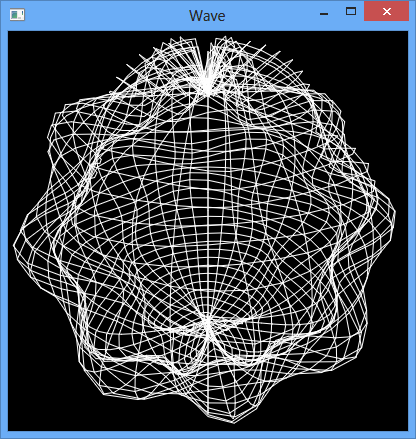
\includegraphics[width=0.5\textwidth]{wave.png}
\end{center}
You are welcome to have the wave actually move (for this purpose there is already a \texttt{time} uniform set up in the shader for you).

Hint: What you want to do is to shift the position of each vertex back and forth according to a sinewave along the direction of the normal at this vertex. The normal direction can be obtained using the \verb#gl_Normal# built-in variable. The phase of the sinewave could depend on the $z$ coordinate of the vertex and/or the \texttt{atan(y, x)} angle. You can also try multiplying sinewaves together to achieve the necessary effect.

Hint: It seems that the \verb#gl_Normal# vectors that FreeGLUT outputs for the vertices of the sphere do not have their fourth element equal to zero (looks like a FreeGLUT bug to me). This may result in unexpected results. To fix this do something like
\begin{verbatim}
  vec4 normal = vec4(gl_Normal.xyz, 0);
\end{verbatim}
\end{exercise}

Note that if you develop a complex scene with several objects, it is completely normal to have a separate shader assigned to each object. For example, you could have several wavy spheres flying around, each with its own ``waviness'' pattern. Conversely, you can also reuse the same shader effect for different objects: try replacing the \verb#glutSolidSphere# with a \verb#glutSolidCylinder#, for example, while keeping the same shader.

\end{document}
